\usepackage[titletoc]{appendix}
\usepackage{xeCJK}
\usepackage{amsmath}
\usepackage{array}
\usepackage{bm}
\usepackage{booktabs}
\usepackage{caption}
\usepackage{cite}
\usepackage{comment}
\usepackage{float}
\usepackage{fontspec} % xelatex限定
\usepackage{geometry}
\usepackage{graphicx}
\usepackage{indentfirst}
% \usepackage[utf8]{inputenc} % 非xelatex编译,显式指定文件编码为utf8
\usepackage{listings}
\usepackage{longtable}
\usepackage{mathtools}
\usepackage{multicol}
\usepackage{multirow}
\usepackage{supertabular}
\usepackage{subcaption}
\usepackage{tabu}
\usepackage{ulem}
\usepackage{url}
\usepackage{xcolor}
\usepackage{nccmath} % だが align* は nccmath が無くても使えるので敢えて両方書いた。
% \usepackage{CJKutf8}
% \usepackage{hyperref}

\geometry{a4paper,left=2.5cm,right=2.5cm,top=2.5cm,bottom=2.5cm}
\defaultCJKfontfeatures{Scale=1.2}
\linespread{1.5}

%% Define a new 'leo' style for the package that will use a smaller font.
\makeatletter
\def\url@leostyle{%
  \@ifundefined{selectfont}{\def\UrlFont{\sf}}{\def\UrlFont{\small\ttfamily}}}
\makeatother
\urlstyle{leo} % Now actually use the newly defined style.


\renewcommand{\contentsname}{\centering{目录}}
\renewcommand{\abstractname}{\large{摘要}}
\def\tablename{表}
\def\figurename{图}
\renewcommand{\thetable}{\thesection.\arabic{table}}
\renewcommand{\thefigure}{\thesection.\arabic{figure}}
\renewcommand{\multirowsetup}{\centering}
\renewcommand{\appendixname}{附录~\Alpha{section}}
\renewcommand{\refname}{参考文献}

\everymath{\displaystyle}
\bibliographystyle{plain}


\lstdefinestyle{BASH}{
    breaklines=true,                                     % 自动换行
    columns=fixed,
    extendedchars=true,                                  % lets you use non-ASCII characters; for 8-bits encodings only, does not work with UTF-8
    frame=shadowbox,                                     % 设置背景边框
    numbers=left,                                        % 在左侧显示行号
    numberstyle=\footnotesize\color{darkgray},           % 设定行号格式
    showstringspaces=false,                              % 不显示字符串中的空格
    tabsize=4,	                                         % 设置tab长度
}
\lstdefinestyle{tinyBASH}{
    breaklines=true,                                     % 自动换行
    basicstyle=\footnotesize\ttfamily,
    columns=fixed,
    extendedchars=true,                                  % lets you use non-ASCII characters; for 8-bits encodings only, does not work with UTF-8
    frame=shadowbox,                                     % 设置背景边框
    numbers=left,                                        % 在左侧显示行号
    numberstyle=\footnotesize\color{darkgray},           % 设定行号格式
    showstringspaces=false,                              % 不显示字符串中的空格
    tabsize=4,	                                         % 设置tab长度
}
\lstdefinestyle{Python}{
    breaklines=true,                                     % 自动换行
    captionpos=b,                                        % sets the caption-position to bottom
    columns=fixed,
    commentstyle=\it\color[RGB]{0,96,96},                % 设置代码注释的格式
    % extendedchars=true,                                  % lets you use non-ASCII characters; for 8-bits encodings only, does not work with UTF-8
    frame=shadowbox,                                     % 设置背景边框
    keywordstyle=\bfseries\color[RGB]{40,40,255},        % 设定关键字颜色
    language=Python,                                     % 设置语言
    numbers=left,                                        % 在左侧显示行号
    numberstyle=\footnotesize\color{darkgray},           % 设定行号格式
    stringstyle=\rmfamily\slshape\color[RGB]{128,0,0},   % 设置字符串格式
    tabsize=4,	                                         % 设置tab长度
}

\lstdefinestyle{CPP}{
    %backgroundcolor=\color[RGB]{245,245,244},           % 设定背景颜色
    breaklines=true,                                     % 自动换行
    captionpos=b,                                        % sets the caption-position to bottom
    columns=fixed,
    commentstyle=\it\color[RGB]{0,96,96},                % 设置代码注释的格式
    extendedchars=true,                                  % lets you use non-ASCII characters; for 8-bits encodings only, does not work with UTF-8
    frame=shadowbox,                                     % 设置背景边框
    keywordstyle=\bfseries\color[RGB]{40,40,255},        % 设定关键字颜色
    language=c++,                                        % 设置语言
    numbers=left,                                        % 在左侧显示行号
    numberstyle=\footnotesize\color{darkgray},           % 设定行号格式
    showstringspaces=false,                              % 不显示字符串中的空格
    stringstyle=\rmfamily\slshape\color[RGB]{128,0,0},   % 设置字符串格式
    tabsize=4,	                                         % 设置tab长度
    title=\lstname,                                      % show the filename of files included with \lstinputlisting; also try caption instead of title
    morekeywords={alignas,continute,friend,register,true,alignof,decltype,goto,
        reinterpret_cast,try,asm,defult,if,return,typedef,auto,delete,inline,short,
        typeid,bool,do,int,signed,typename,break,double,long,sizeof,union,case,
        dynamic_cast,mutable,static,unsigned,catch,else,namespace,static_assert,using,
        char,enum,new,static_cast,virtual,char16_t,char32_t,explict,noexcept,struct,
        void,export,nullptr,switch,volatile,class,extern,operator,template,wchar_t,
        const,false,private,this,while,constexpr,float,protected,thread_local,
        const_cast,for,public,throw,std},
    emph={map,set,multimap,multiset,unordered_map,unordered_set,
        unordered_multiset,unordered_multimap,vector,string,list,deque,
        array,stack,forwared_list,iostream,memory,shared_ptr,unique_ptr,
        random,bitset,ostream,istream,cout,cin,endl,move,default_random_engine,
        uniform_int_distribution,iterator,algorithm,functional,bing,numeric},
}

\lstdefinestyle{QT}{
    %backgroundcolor=\color[RGB]{245,245,244},           % 设定背景颜色
    breaklines=true,                                     % 自动换行
    captionpos=b,                                        % sets the caption-position to bottom
    columns=fixed,
    commentstyle=\it\color[RGB]{0,96,96},                % 设置代码注释的格式
    extendedchars=true,                                  % lets you use non-ASCII characters; for 8-bits encodings only, does not work with UTF-8
    frame=shadowbox,                                     % 设置背景边框
    keywordstyle=\bfseries\color[RGB]{40,40,255},        % 设定关键字颜色
    language=c++,                                        % 设置语言
    numbers=left,                                        % 在左侧显示行号
    numberstyle=\footnotesize\color{darkgray},           % 设定行号格式
    stringstyle=\rmfamily\slshape\color[RGB]{128,0,0},   % 设置字符串格式
    showstringspaces=false,                              % 不显示字符串中的空格
    tabsize=4,	                                         % 设置tab长度
    title=\lstname,                                      % show the filename of files included with \lstinputlisting; also try caption instead of title
    morekeywords={alignas,continute,friend,register,true,alignof,decltype,goto,
        reinterpret_cast,try,asm,defult,if,return,typedef,auto,delete,inline,short,
        typeid,bool,do,int,signed,typename,break,double,long,sizeof,union,case,
        dynamic_cast,mutable,static,unsigned,catch,else,namespace,static_assert,using,
        char,enum,new,static_cast,virtual,char16_t,char32_t,explict,noexcept,struct,
        void,export,nullptr,switch,volatile,class,extern,operator,template,wchar_t,
        const,false,private,this,while,constexpr,float,protected,thread_local,
        const_cast,for,public,throw,std,bind,function,
        Q_OBJECT,QDialog,QUdpSocket,QTcpSocket,QHostAddress,QNetworkDatagram,QTcpServer,
        QByteArray,QString,QStringList,QList,QSet,QMap,
        quint,qint64,uintptr_t,
        connect,signals,slots,SIGNAL,SLOT},
    emph={map,set,multimap,multiset,unordered_map,unordered_set,
        unordered_multiset,unordered_multimap,vector,string,list,deque,
        array,stack,forwared_list,iostream,memory,shared_ptr,unique_ptr,
        random,bitset,ostream,istream,cout,cin,endl,move,default_random_engine,
        uniform_int_distribution,iterator,algorithm,functional,bing,numeric},
}

\lstdefinestyle{MASM}{
    breaklines=true,                                     % 自动换行
    captionpos=b,                                        % sets the caption-position to bottom
    columns=fixed,
    commentstyle=\it\color[RGB]{0,96,96},                % 设置代码注释的格式
    extendedchars=true,                                  % lets you use non-ASCII characters; for 8-bits encodings only, does not work with UTF-8    
    frame=shadowbox,                                     % 设置背景边框
    keywordstyle=\bfseries\color[RGB]{40,40,255},        % 设定关键字颜色
    language=[x86masm]Assembler,                         % 设置语言
    numbers=left,                                        % 在左侧显示行号
    numberstyle=\footnotesize\color{darkgray},           % 设定行号格式
    stringstyle=\rmfamily\slshape\color[RGB]{128,0,0},   % 设置字符串格式
    showstringspaces=false,                              % 不显示字符串中的空格
    tabsize=4,	                                         % 设置tab长度
    title=\lstname,                                      % show the filename of files included with \lstinputlisting; also try caption instead of title
    morekeywords={CDQE,CQO,CMPSQ,CMPXCHG16B,JRCXZ,LODSQ,MOVSXD, % 
        POPFQ,PUSHFQ,SCASQ,STOSQ,IRETQ,RDTSCP,SWAPGS, % 
        .code,.def,.file,.type,.ended,.scl,.section,.ascii,.text,.globl,.ident,.rodata,
        .sch_proc,.sch_pushreg,.sch_setframe,.sch_stackalloc,.sch_endprologue,.sch_endproc,
        pushq,popq,movq,movl,addq,subq,leaq,invoke,start,addr,
        rax,rdx,rcx,rbx,rsi,rdi,rip,rsp,rbp, % 
        r8,r8d,r8w,r8b,r9,r9d,r9w,r9b, % 
        r10,r10d,r10w,r10b,r11,r11d,r11w,r11b, % 
        r12,r12d,r12w,r12b,r13,r13d,r13w,r13b, % 
        r14,r14d,r14w,r14b,r15,r15d,r15w,r15b}
}
\newcommand{\includecode}[2][c]{\lstinputlisting[caption=#2, escapechar=, style=#1]{#2}}



% \setcounter{table}{0}
% \setcounter{figure}{0}

% \lstinputlisting[style=CPP]{src/main.cpp}

% \begin{figure}[H]
%     \centering
%     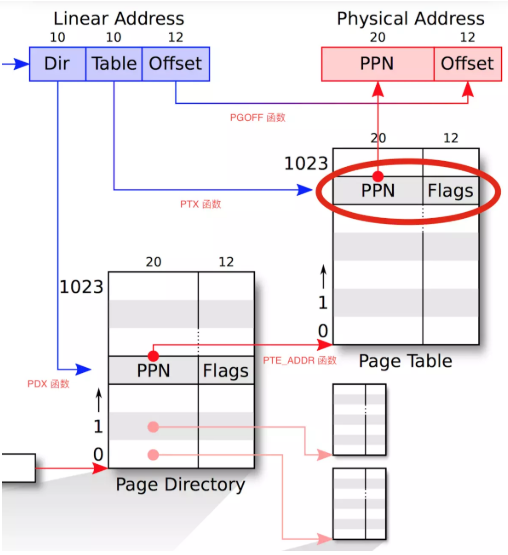
\includegraphics[width = .75\linewidth]{img/1.png}
%     \caption{预处理结果(部分)}
%     \label{fig::figure2}
% \end{figure}


% 结果如表\ref{tab::table2}:
% \begin{table}[htbp]
%     \begin{center}
%         \begin{tabular}{c c c}
%             \toprule
%             优化等级 & 二进制文件大小(Byte) &  执行时间(s)\\
%             \midrule
%             不优化 & 13992 & 36.090 \\
%             O1 & 13344 & 10.562\\
%             O2 & 13344 & 9.925\\
%             Os & 13344 & 8.899\\
%             O3 & 13344 & 8.350\\
%             Ofast & 14800 & 8.094\\
%             \bottomrule
%         \end{tabular}
%         \caption{各等级优化测试结果}\label{tab::table2}
%     \end{center}
% \end{table}

% \begin{equation}
%     \begin{split}
%         id     & \rightarrow char\ |\ id\ digit\ |\ id\ char \\
%         digit  & \rightarrow 0\ |\ 1\ |\ 2\ |\ 3\ |\ 4\ |\ 5\ |\ 6\ |\ 7\ |\ 8\ |\ 9 \\
%         char   & \rightarrow \_\ |\ letter \\
%         letter & \rightarrow A\ |\ B\ |\ ...\ |\ Z\ |\ a\ |\ b\ |\ ...\ |\ z \\
%     \end{split}
% \end{equation}